\section{Temperature dependence of rate coefficients}
\label{subsec:temp-dependence}

This section briefly discusses the temperature dependence of the ternary
association and collision-induced dissociation of \CD ion with He buffer gas.
As discussed in Section \ref{subsec:rate-constants}, Figure
\ref{fig:off:rate-constants:f(t)} shows the experimentally measured formation
($k_{3_1}$) and collision dissociation ($k_{CID_1}$) rate coefficient plotted
as a function of temperature (T$_{trap}$). The subscript $1$ corresponds to the
first complex, i.e., He\CD. As depicted in the figure, the $k_{3_1}$ and
$k_{CID_1}$ increase as the temperature increases.

\begin{figure}[!htb]
    \centering
    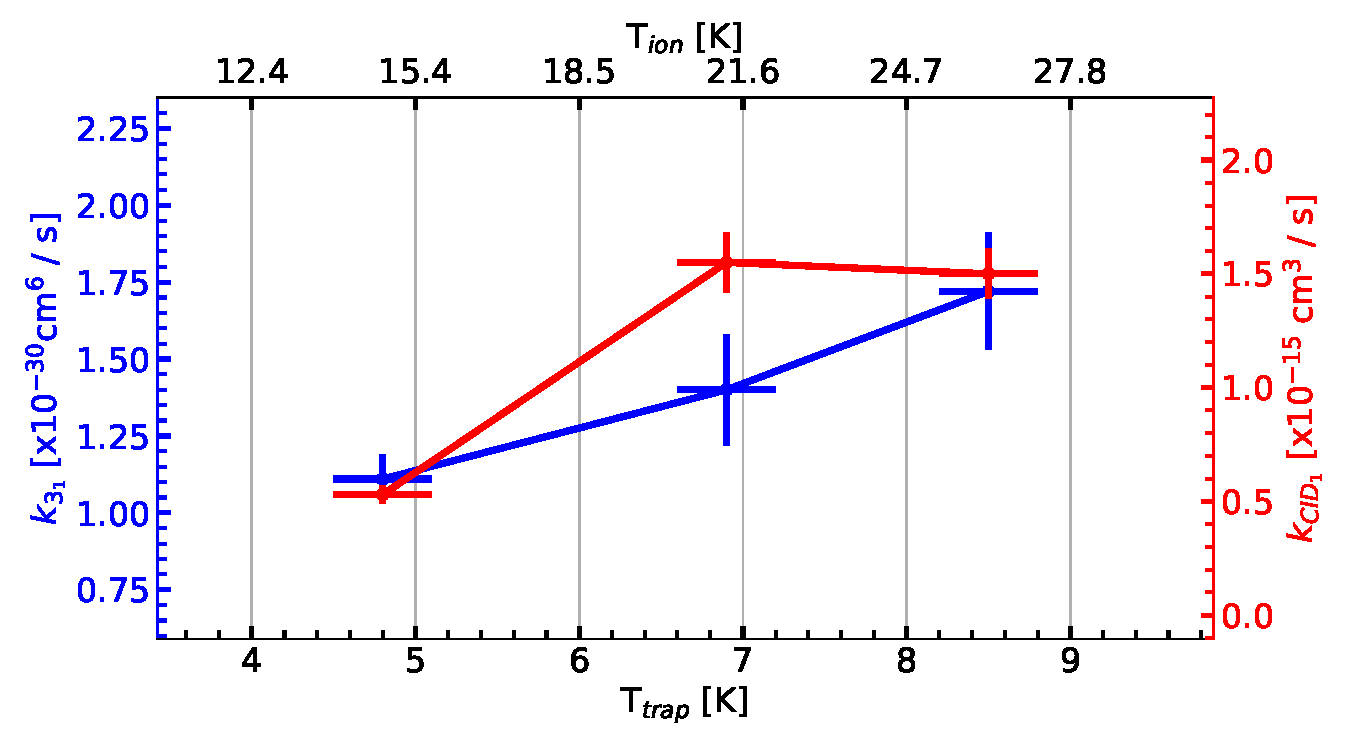
\includegraphics[width=1\textwidth]{figures/measurements/kinetics/functionOf_T/off_k3_kCID_as_functionOfT_with_Tcol.pdf}
    \caption{He\CD The formation (\textcolor{blue}{$k_{3_1}$}) and dissociation (\textcolor{red}{$k_{CID_1}$}) rate constants (weighted) are plotted as a function of nominal trap temperature (T$_{trap}$) and ion temperature (T$_{ion}$). The x-axis error bar corresponds to T$_{trap}$. }
    \label{fig:off:rate-constants:f(t)}
\end{figure}

The dissociation rates are collision-induced. The reaction cross-section gives
the probability of ion and neutral collision. Thus, the rate coefficients are
derived by multiplying the cross-section with a relative velocity of reactants
followed by averaging over a Maxwell-Boltzmann distribution. So, as the
temperature increases, the collisional velocity and energy increase, which
increases $k_{CID}$ rate coefficients.

However, the formation rates, especially for the ternary association reactions
between ions and neutrals at a low temperature, possess an inverse temperature
dependence because of a decrease in the effective probability of forming a
stable complex with a single collision \cite{herbst_dense_1988} (see Section
\ref{subsec:rate-theory} for two-step process). This contrasts our observation
as shown in Figure \ref{fig:off:rate-constants:f(t)}. The ternary rate
temperature dependence of $k_3 (\text{T}) \propto \text{T}^{-3/4}$ was obtained
back in the 1960s by \citet{smirnov_transitions_1967} for ion-neutral
three-body association reactions at temperatures $>100$ K. The same dependence
was also shown in recent studies based on the classical trajectory approach
\cite{perez-rios_communication_2015, greene_universal_2017}.

\citet{bohringer_temperature_1983} experimentally investigated the temperature dependence ($30-300$ K) of He$_2^+$ formation via ternary association using a cryogenic selected ion drift tube, i.e., similar a ion-neutral reaction, but He$^+$ ion is investigated instead of molecular \CD, as shown below:

\begin{equation}
    \text{He}^+ + 2\text{He} \rightarrow \text{He}_2^+ + \text{He}
    \label{eqn:He2+-ternary}
\end{equation}

They observed an inverse temperature dependence and derived a relation for Eq.
\ref{eqn:He2+-ternary}, such as:

\begin{equation}
    k_3 (\text{T}) = 1.4 \times 10^{-31} (300 \text{ K} / \text{T})^{0.6} \text{ cm}^6\text{s}^{-1}
    \label{eqn:k3(T)-dependence}
\end{equation}

\citet{gerlich_experimental_1993} and Pla\v{s}il, et al. \cite{plasil_stabilization_2012} performed the same He$_2^+$ experiment but using a ring electrode trap and 22-pole cryogenic ion trap, respectively. They showed the inverse temperature dependence for $k_3$ at T$_{trap}>10$ K that agrees with the equation \ref{eqn:k3(T)-dependence}.\\

In order to investigate if the discrepancy stems from the fact that we use a
molecular ion, or if the observed increase might stem from a reaction-specific
resonance in the attachment process, we repeated the measurement but now with
N$^+$, i.e.,

\[ \text{N}^+ + 2\text{He} \rightarrow \text{NHe}^+ + \text{He}\]

The N$^+$ ion has the same $m/z\ 14$ as \CD. The experimental procedure is
similar to the one described in Section \ref{sec:CD+-kinetics}. The derived
formation and dissociative rate coefficients are shown in Figure
\ref{fig:rate-constants:N+} (in appendix) for a temperature T$_{trap}=5-10$ K
and a pressure range from $(1 - 9 ) \cdot 10^{14}$\percc. The temperature
dependence plot for $k_3$ and $k_{CID}$ for N$^+$+2He reaction is shown in
Figure \ref{fig:HeN+:rate-constants-f(t)}.

\begin{figure}[!htb]
    \centering
    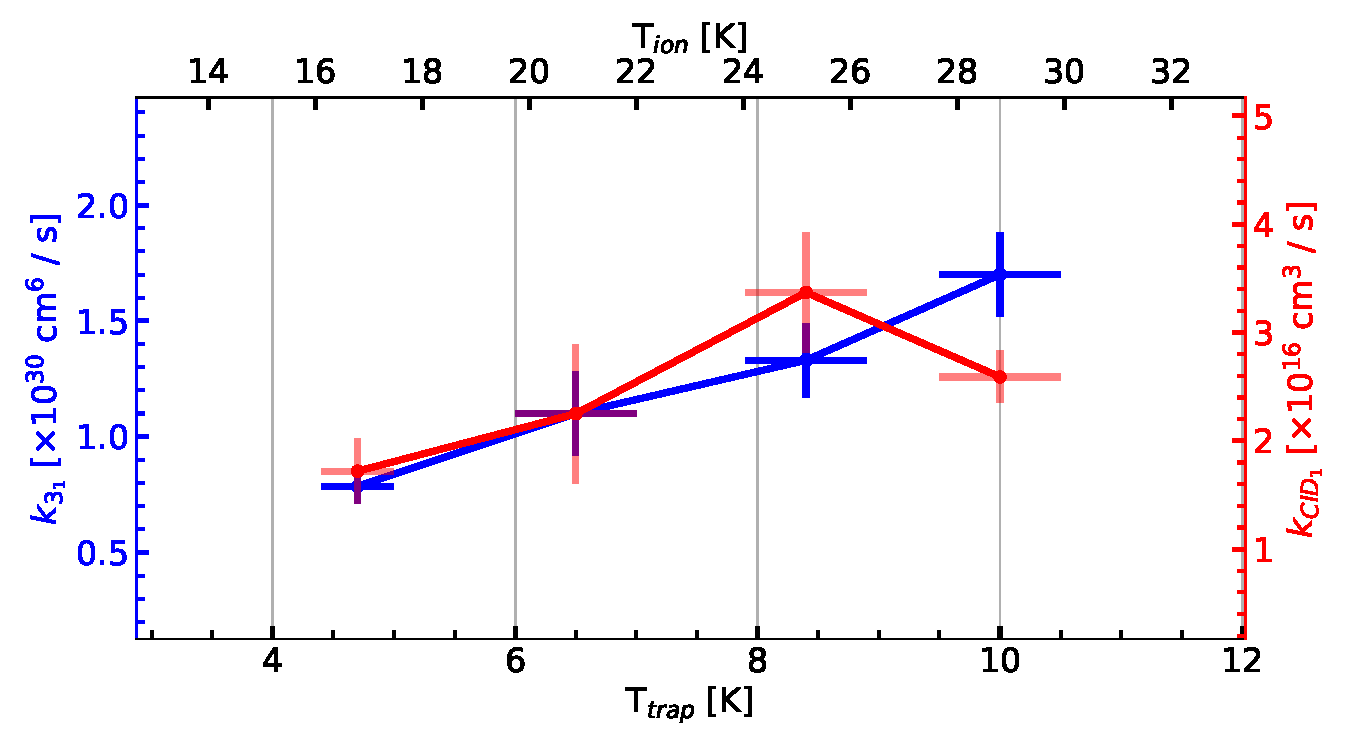
\includegraphics[width=1\textwidth]{figures/measurements/kinetics/functionOf_T/N+/off_k3_kCID_as_functionOfT_with_Tcol.pdf}
    \caption{HeN$^+$ formation (\textcolor{blue}{$k_{3_1}$}) and dissociation (\textcolor{red}{$k_{CID_1}$}) rate constants (weighted) are plotted as a function of nominal trap temperature. The T$_{ion}$ indicated here is measured for the \CD ion which has the same m/z 14.}
    \label{fig:HeN+:rate-constants-f(t)}
\end{figure}

\begin{table}[!htb]
    \centering
    \caption{Formation ($k_{3_1}$) and dissociation ($k_{CID_1}$) rate constants for N$^+$ and \CD reactions with helium at different nominal trap temperature}. 
    \begin{tabular}{c|cccc}
        \hline\\
        &\multicolumn{2}{c}{$k_{3_1}$ [cm$^6$s$^{-1}$]} &\multicolumn{2}{c}{$k_{CID_1}$ [cm$^3$s$^{-1}$]} \\
        & \multicolumn{2}{c}{$\times 10^{-30}$} & \multicolumn{2}{c}{$\times 10^{-16}$}\\
        T$_{trap}$ [K] & N$^+$ & \CD & N$^+$ & \CD \\
        \\\hline\hline\\
        4.7(3)  & 0.80(1) & 1.1(1) & 1.7(1) &  5.3(0.4)  \\
        6.5(5)  & 1.1(1)  & 1.4(2) & 2.2(2) & 15.5(1.3)  \\
        8.4(5)  & 1.4(1)  & 1.7(2) & 3.4(3) & 15.0(1.1)  \\
        10.0(5) & 1.7(1)  & -      & 2.5(2) & -  \\
        \\\hline\hline\\
    \end{tabular}
    \label{tab:k3:rate-constants-T-depen}
\end{table}

Surprisingly, similar to \CD ion, the N$^+$ molecular ion also shows the same increasing trend for ternary association reaction. The measured ternary association and collision-induced dissociation rate coefficients are summarised in Table \ref{tab:k3:rate-constants-T-depen}.

However, most experiments previously performed, including the study on He$^+$
previously discussed above are performed at temperatures $>10$ K.
Interestingly, \citet{gerlich_infrared_2018} again investigated the He$_2^+$
formation (see Eq. \ref{eqn:He2+-ternary}) using a 22-pole cryogenic ion trap
but at T$_{trap}=4$ K temperature. But unlike the experiments at $>10$ K (see
above), this disagrees (i.e., $k_3$ is lower at a lower temperature) with the
relation as shown in equation \ref{eqn:k3(T)-dependence}.

\citet{xie_quantum_2003} performed a quantum dynamical study for the same He$_2^+$ formation reaction via three-body association (Eq. \ref{eqn:He2+-ternary}). They reported that the ternary association rate coefficient dramatically increases with temperature, i.e., $k_3(\text{T}) \propto \text{T}$, but only at temperatures below $< 30$ K, then they drop down after reaching a maximum value. They argued that this behaviour is because, up to a certain low temperature, the population of quantum states of ions contributing to a resonance state promoting complex formation increases with temperature, thus increasing in $k_3$. This also indicates that the particular ion-neutral reaction proceeds via a two-step mechanism as discussed in Section \ref{subsec:rate-theory}.

In order to verify if the complex formation for He\CD and HeN$^+$ also proceeds
via a resonance state, theoretical calculations need to be performed. First
quasi-classical scattering calculations cannot reproduce the observed
temperature dependence (J. Perez-Rios, private communication), so full quantum
scattering calculations are likely needed. The fact that both temperature
curves (for N$^+$ and \CD) show the same behaviour, might also indicate an
experimental artefact, e.g., periodic freezing out of He to the trap walls due
to the 1s duty cycle of the cryostat. In the future, we would like to repeat
the He$_2^+$ reaction at low temperatures in our apparatus and compare the
results to literature values \cite{bohringer_temperature_1983,
    plasil_stabilization_2012, gerlich_infrared_2018}.

% However, from the experimental point of view, one could also argue that this could have something to do with the 22-pole ion trap. Nevertheless, in conclusion, we need to compare our experimental data with theoretical methods for low-temperature \CD and N$^+$ with He measurements to have conclusive evidence, which is planned in future studies.